% Options for packages loaded elsewhere
% Options for packages loaded elsewhere
\PassOptionsToPackage{unicode}{hyperref}
\PassOptionsToPackage{hyphens}{url}
\PassOptionsToPackage{dvipsnames,svgnames,x11names}{xcolor}
%
\documentclass[
  letterpaper,
  DIV=11,
  numbers=noendperiod]{scrartcl}
\usepackage{xcolor}
\usepackage{amsmath,amssymb}
\setcounter{secnumdepth}{-\maxdimen} % remove section numbering
\usepackage{iftex}
\ifPDFTeX
  \usepackage[T1]{fontenc}
  \usepackage[utf8]{inputenc}
  \usepackage{textcomp} % provide euro and other symbols
\else % if luatex or xetex
  \usepackage{unicode-math} % this also loads fontspec
  \defaultfontfeatures{Scale=MatchLowercase}
  \defaultfontfeatures[\rmfamily]{Ligatures=TeX,Scale=1}
\fi
\usepackage{lmodern}
\ifPDFTeX\else
  % xetex/luatex font selection
\fi
% Use upquote if available, for straight quotes in verbatim environments
\IfFileExists{upquote.sty}{\usepackage{upquote}}{}
\IfFileExists{microtype.sty}{% use microtype if available
  \usepackage[]{microtype}
  \UseMicrotypeSet[protrusion]{basicmath} % disable protrusion for tt fonts
}{}
\makeatletter
\@ifundefined{KOMAClassName}{% if non-KOMA class
  \IfFileExists{parskip.sty}{%
    \usepackage{parskip}
  }{% else
    \setlength{\parindent}{0pt}
    \setlength{\parskip}{6pt plus 2pt minus 1pt}}
}{% if KOMA class
  \KOMAoptions{parskip=half}}
\makeatother
% Make \paragraph and \subparagraph free-standing
\makeatletter
\ifx\paragraph\undefined\else
  \let\oldparagraph\paragraph
  \renewcommand{\paragraph}{
    \@ifstar
      \xxxParagraphStar
      \xxxParagraphNoStar
  }
  \newcommand{\xxxParagraphStar}[1]{\oldparagraph*{#1}\mbox{}}
  \newcommand{\xxxParagraphNoStar}[1]{\oldparagraph{#1}\mbox{}}
\fi
\ifx\subparagraph\undefined\else
  \let\oldsubparagraph\subparagraph
  \renewcommand{\subparagraph}{
    \@ifstar
      \xxxSubParagraphStar
      \xxxSubParagraphNoStar
  }
  \newcommand{\xxxSubParagraphStar}[1]{\oldsubparagraph*{#1}\mbox{}}
  \newcommand{\xxxSubParagraphNoStar}[1]{\oldsubparagraph{#1}\mbox{}}
\fi
\makeatother


\usepackage{longtable,booktabs,array}
\usepackage{calc} % for calculating minipage widths
% Correct order of tables after \paragraph or \subparagraph
\usepackage{etoolbox}
\makeatletter
\patchcmd\longtable{\par}{\if@noskipsec\mbox{}\fi\par}{}{}
\makeatother
% Allow footnotes in longtable head/foot
\IfFileExists{footnotehyper.sty}{\usepackage{footnotehyper}}{\usepackage{footnote}}
\makesavenoteenv{longtable}
\usepackage{graphicx}
\makeatletter
\newsavebox\pandoc@box
\newcommand*\pandocbounded[1]{% scales image to fit in text height/width
  \sbox\pandoc@box{#1}%
  \Gscale@div\@tempa{\textheight}{\dimexpr\ht\pandoc@box+\dp\pandoc@box\relax}%
  \Gscale@div\@tempb{\linewidth}{\wd\pandoc@box}%
  \ifdim\@tempb\p@<\@tempa\p@\let\@tempa\@tempb\fi% select the smaller of both
  \ifdim\@tempa\p@<\p@\scalebox{\@tempa}{\usebox\pandoc@box}%
  \else\usebox{\pandoc@box}%
  \fi%
}
% Set default figure placement to htbp
\def\fps@figure{htbp}
\makeatother


% definitions for citeproc citations
\NewDocumentCommand\citeproctext{}{}
\NewDocumentCommand\citeproc{mm}{%
  \begingroup\def\citeproctext{#2}\cite{#1}\endgroup}
\makeatletter
 % allow citations to break across lines
 \let\@cite@ofmt\@firstofone
 % avoid brackets around text for \cite:
 \def\@biblabel#1{}
 \def\@cite#1#2{{#1\if@tempswa , #2\fi}}
\makeatother
\newlength{\cslhangindent}
\setlength{\cslhangindent}{1.5em}
\newlength{\csllabelwidth}
\setlength{\csllabelwidth}{3em}
\newenvironment{CSLReferences}[2] % #1 hanging-indent, #2 entry-spacing
 {\begin{list}{}{%
  \setlength{\itemindent}{0pt}
  \setlength{\leftmargin}{0pt}
  \setlength{\parsep}{0pt}
  % turn on hanging indent if param 1 is 1
  \ifodd #1
   \setlength{\leftmargin}{\cslhangindent}
   \setlength{\itemindent}{-1\cslhangindent}
  \fi
  % set entry spacing
  \setlength{\itemsep}{#2\baselineskip}}}
 {\end{list}}
\usepackage{calc}
\newcommand{\CSLBlock}[1]{\hfill\break\parbox[t]{\linewidth}{\strut\ignorespaces#1\strut}}
\newcommand{\CSLLeftMargin}[1]{\parbox[t]{\csllabelwidth}{\strut#1\strut}}
\newcommand{\CSLRightInline}[1]{\parbox[t]{\linewidth - \csllabelwidth}{\strut#1\strut}}
\newcommand{\CSLIndent}[1]{\hspace{\cslhangindent}#1}



\setlength{\emergencystretch}{3em} % prevent overfull lines

\providecommand{\tightlist}{%
  \setlength{\itemsep}{0pt}\setlength{\parskip}{0pt}}



 


\usepackage{amsmath}
\KOMAoption{captions}{tableheading}
\makeatletter
\@ifpackageloaded{caption}{}{\usepackage{caption}}
\AtBeginDocument{%
\ifdefined\contentsname
  \renewcommand*\contentsname{Table of contents}
\else
  \newcommand\contentsname{Table of contents}
\fi
\ifdefined\listfigurename
  \renewcommand*\listfigurename{List of Figures}
\else
  \newcommand\listfigurename{List of Figures}
\fi
\ifdefined\listtablename
  \renewcommand*\listtablename{List of Tables}
\else
  \newcommand\listtablename{List of Tables}
\fi
\ifdefined\figurename
  \renewcommand*\figurename{Figure}
\else
  \newcommand\figurename{Figure}
\fi
\ifdefined\tablename
  \renewcommand*\tablename{Table}
\else
  \newcommand\tablename{Table}
\fi
}
\@ifpackageloaded{float}{}{\usepackage{float}}
\floatstyle{ruled}
\@ifundefined{c@chapter}{\newfloat{codelisting}{h}{lop}}{\newfloat{codelisting}{h}{lop}[chapter]}
\floatname{codelisting}{Listing}
\newcommand*\listoflistings{\listof{codelisting}{List of Listings}}
\makeatother
\makeatletter
\makeatother
\makeatletter
\@ifpackageloaded{caption}{}{\usepackage{caption}}
\@ifpackageloaded{subcaption}{}{\usepackage{subcaption}}
\makeatother
\usepackage{bookmark}
\IfFileExists{xurl.sty}{\usepackage{xurl}}{} % add URL line breaks if available
\urlstyle{same}
\hypersetup{
  pdftitle={Notes on Spark Project},
  pdfauthor={Paulinha},
  colorlinks=true,
  linkcolor={blue},
  filecolor={Maroon},
  citecolor={Blue},
  urlcolor={Blue},
  pdfcreator={LaTeX via pandoc}}


\title{Notes on Spark Project}
\author{Paulinha}
\date{}
\begin{document}
\maketitle


\section{Overview}\label{overview}

Costs and benefits are inherent aspects of species interactions. Costs
associated with mutualistic interactions, such as pollination and seed
dispersal, involve production of nectar and fruit from a plant
perspective and from an animal perspective there are costs associated
with finding and acquiring nectar as well as digesting and processing
fruits. The benefits are associated with the provision of resources to
the animals and the reproduction to plants. Beyond the importance of the
mutualistic interactions to the persistence of interacting species,
these interactions also provide ecosystem services, such as production
of crops and landscape connectivity. The costs and benefits associated
with species interactions are not fixed and are subjected to changes due
to environmental conditions, which scale up affecting the provision of
ecosystem services.

We developed a framework to explore how costs and benefits associated
with species interactions, and consequently ecosystem services,
determine the persistence of species and the robustness of service
provision under environmental changes. Our modeling framework combines
cost-benefit analysis defining fitness functions that determines the
outcome of a Boolean process. The Boolean process establishes which
species are present in the community given the costs and benefit
associated with interactions between species. The presence of species
determines whether ecosystem services will be provided. Our model
detects transition phases in mutualisms based on increasing costs of
interactions associated with environmental changes. We explored how
network structure influences species persistence and ecosystem services
provision with both theoretical random networks as well as networks
parameterized using empirical data for different sampled cost/benefit
functions.

Given the broad nature of the modeling framework we took two
complementary approaches. Within the first approach we explored how the
processes incorporated in the model lead to network structures that
resemble empirical ones. The second approach takes empirical networks as
a starting point and explores the consequences of the processes
incorporated in the model to the persistence of mutualisms and ecosystem
services. These two approaches are explored concomitantly and attack (i)
how processes lead to patterns and (ii) the consequences of processes in
the emerging patterns.

\section{Methods}\label{methods}

The two approaches share the same modeling framework's backbone. The
common shared aspects of both projects are presented below and
afterwards each approach described its own questions and peculiarities.
In both cases, a bipartite network of interacting species is defined
(either theoretically or empirically). The two sets of nodes can
represent plants and pollinators and/or plants and frugivores.
Interactions are established between nodes from different sets and each
interaction is associated with costs and benefits. The balance between
costs and benefits defines which species will be present in the
community following a decision function.

\subsection{Interaction networks}\label{interaction-networks}

The proposed modeling framework is a benchmark to understand how
distributions of costs and benefits associated with the interactions
influences community structure and persistence of species. Starting from
a pool of potential interacting species from two groups (i.e., a
bipartite structure of plants and pollinators, for example), we assume
all species can potentially interact, given a certain connectance and an
underlying model to define which species interact. Once interactions are
established, we define the costs and benefits associated with each
interaction for each partner.

\subsection{Cost and benefit
functions}\label{cost-and-benefit-functions}

The costs and benefits associated with the interactions between species
follow an underlying distribution. We used the beta distribution, which
is defined on the interval \([0,1]\) in terms of two parameters
\(\alpha\) and \(\beta\) and can take diverse shapes, allowing the
exploration of a diverse array of combinations of costs and benefits.
Additionally, it provides a limit to the maximum benefit (cost) a
species can have. The upper limit is \(k\) (the degree of the species,
assuming it receives the maximum benefit from all its partners, as
benefits are an additive function -- see
Sec.\phantomsection\label{decision-function}{Decision function}). The
beta distribution was used previously to model trophic and competitive
interactions (Cattin et al. 2004; Dunne et al. 2008; Stouffer et al.
2005; Fowler 2010).

Each pairwise interaction is hence associated with an underlying cost
and an underlying benefit, which might follow different
parameterizations from a beta distribution. The balance between costs
and benefits defined by the decision function determines whether a
species is able to persist in a community.

\subsection{Decision Function}\label{decision-function}

Our framework considers a Boolean network determining whether species
persist in their environment given the costs and benefits associated
with the interactions they establish with mutualistic partners, as well
as a contribution of physiological costs associated with the
environment. The existence of costs and benefits depends on the presence
of an interaction encoded in the adjacency matrix that defines which
species interact with whom. The decision function for species \(i\) is
defined as follows:

{[} w\_i = \underbrace{\sum_j(B_{ij} - C_{ij})}\emph{\text{biotic} -
\underbrace{\alpha P_i}}\text{abiotic} {]}

where \(B_{ij}\) is the element \(ij\) of the matrix \(B\) that encodes
the benefits, similarly \(C_{ij}\) is the element \(ij\) of the matrix
\(C\) that encodes the costs of the interaction, both sampled from beta
distributions. For each pairwise interaction, a net benefit is estimated
and summed across all interaction partners, which is the biotic
component of the decision function. \(P_i\) is the physiological cost
associated with the baseline survival of species \(i\) and parameter
\(\alpha\) is the environmental effect, which in combination with the
physiological cost compose the abiotic component of the decision
function. Whenever \(w_i > 0\) species \(i\) persists in the
environment, whereas whenever \(w_i \leq 0\) species \(i\) goes extinct.

\subsection{The Ecosystem-Services
Matrix}\label{the-ecosystem-services-matrix}

The matrix describing the ecosystem services is composed of services on
the rows and species contributing to the services as its columns. This
view of multiple species contributing to an ecosystem service recognizes
that services are built through species acting as providers of the
service per se and species playing a supporting role in the service
(Keyes et al. 2021). The structure of the ecosystem service matrix can
be explored from a theoretical point of view as well as using specific
case studies. For instance, we can connect the structure of the
empirical network of interactions with the structure of the ecosystem
services matrix, where species that play a central role in the matrix
are associated with certain services whereas species in the periphery of
the network are associated with other services. In this example we
further explore how these services differ in their robustness to
species' loss or to environmental changes.

\section{Results}\label{results}

\subsection{Model setting and random
expectations}\label{model-setting-and-random-expectations}

The first part of the projects focuses on the effects of the
distribution of costs and benefits on the persistence of species
interacting in random bipartite networks, following the Erdös-Renyi (ER)
model. The system is initialized with \(n_i\) species in one set and
\(n_j\) species in the other set. Interactions are established between
species belonging to different sets, and the probability of an
interaction between species from different sets is given by \(p\), which
is the expected connectance under the ER-model. Following the Boolean
rules, we explored the proportion of surviving species given the
difference between the first moment of the distribution of costs and of
benefits, i.e., given the difference in the expected values of benefits
\(E[B]\) and costs \(E[C]\). For the beta distribution, this difference
(\(d\)) is given by:

\[
d = E[B] - E[C]
\] \[
E[B]=\frac{\alpha_b}{\alpha_b+\beta_b} 
\] \[
E[C]=\frac{\alpha_c}{\alpha_c+\beta_c} 
\]

When the difference is negative (\(d<0\)), expected costs surpass the
expected benefits for species interactions, and hence, we expect more
species to go extinct. Alternatively, when \(d>0\) the expected benefits
are greater than the expected cost, allowing a greater number of species
to coexist.

\begin{figure}[htbp!]
    \centering
    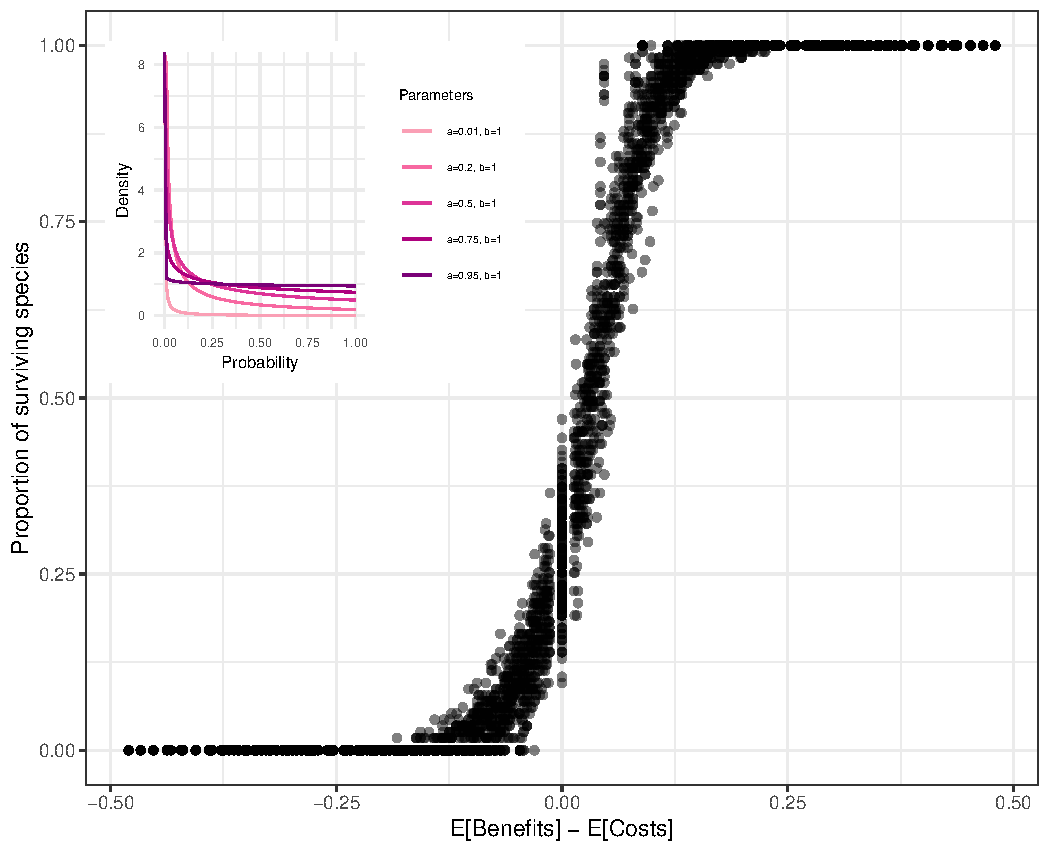
\includegraphics[width=0.5\linewidth]{../src/Code/R/Paulinha/figures/beta1.pdf}
    \caption{Proportion of surviving species given the difference between the expected value of benefits and costs under beta parameterization considering $\beta = 1$ and $0.01 < \alpha< 0.99$. The inset shows the shape of the distribution for different values of $\alpha$ when $\beta =1$. The model was run with random networks consisting of 115 nodes (50 on one set of species and 65 on the other set) and expected connectance of $p=0.65$. Each combination of $\alpha_b$ (associated with benefits) and $\alpha_c$ (associated with costs) had 10 replicates and the proportion of surviving species was recorded.}
    \label{fig:surviving}
\end{figure}

Figure \ref{fig:surviving} shows whenever expected costs are greater
than expected benefits (negative values on the \(x\)-axis), all species
go extinct. As the difference decreases, an increasing proportion of
species remain in the system. Finally, when expected benefits are much
greater than expected costs (positive values on the \(x\)-axis), all
species remain in the system. This pattern holds for other
parameterizations of the beta distribution \ref{fig:alternative_beta},
and alternative choice of distribution (e.g., Lognormal distribution).

\begin{figure}[h]
    \centering
    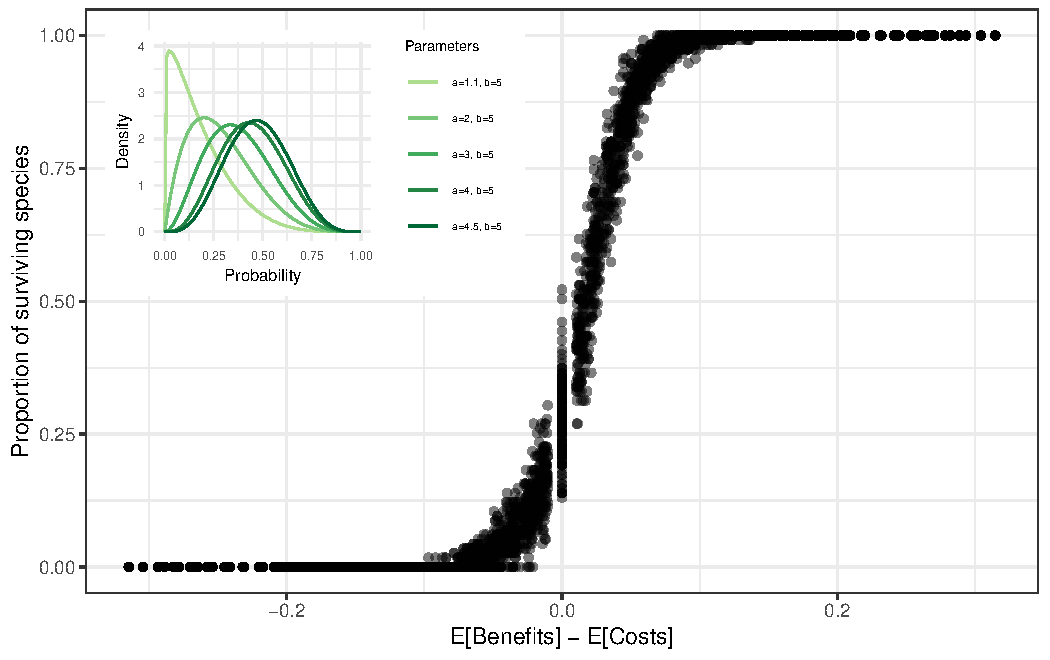
\includegraphics[width=0.48\textwidth]{../src/Code/R/Paulinha/figures/beta2.pdf}
    \hfill
    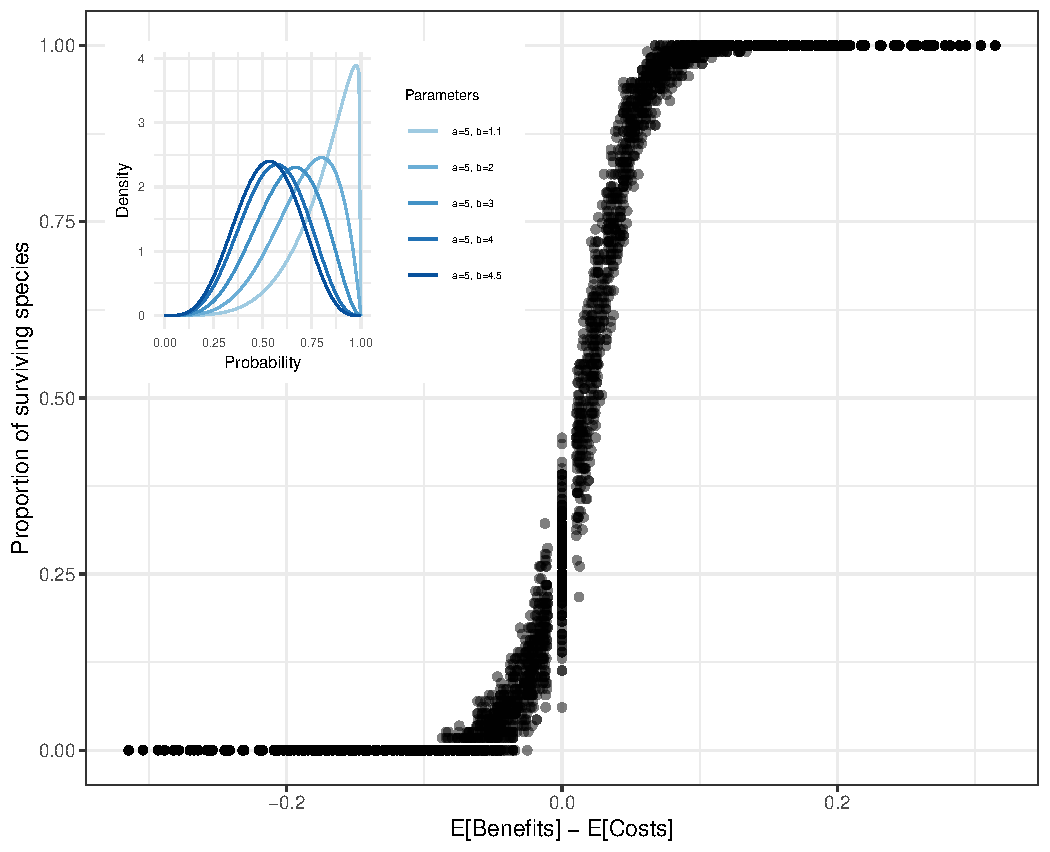
\includegraphics[width=0.48\textwidth]{../src/Code/R/Paulinha/figures/beta3.pdf}
    \caption{Proportion of surviving species given the difference between expected value of benefits and expected value of costs under beta distributions with parameters following the inset graphs.}
    \label{fig:alternative_beta}
\end{figure}

When modeling costs and benefits using a Lognormal distribution. In this
case, the expected values are given by
\(E[X] = e^{(\mu+\frac{\sigma^2}{2})}\). For the lognormal distribution,
there is a greater variance in the range of parameter values leading to
coexistence than observed for the beta distribution. Even with a greater
variance, both distributions lead to an \(S-\)shaped pattern on the
probability of coexistence. These analyses suggest a robust pattern in
how asymmetries in the distribution of costs and benefits shape species
coexistence.

\begin{figure}[h!]
    \centering
    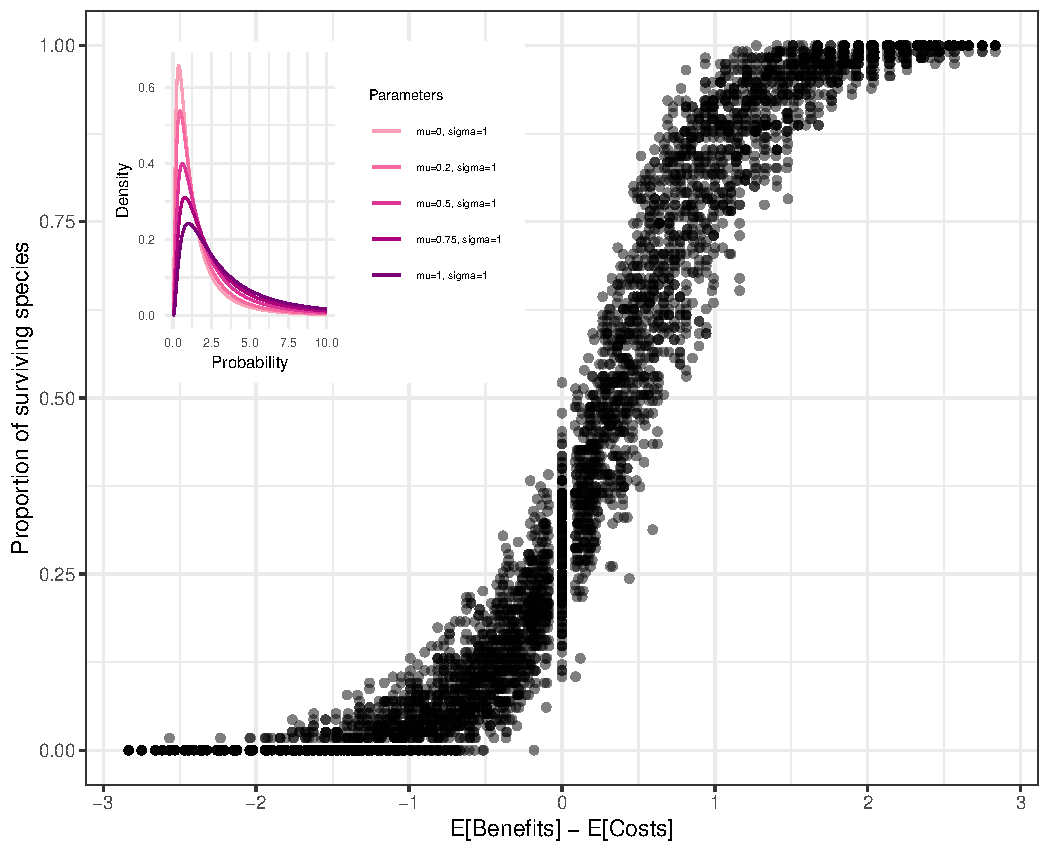
\includegraphics[width=0.5\textwidth]{../src/Code/R/Paulinha/figures/lognorm.pdf}
    \caption{Proportion of surviving species given the difference between expected value of benefits and expected value of costs under lognormal distribution with parameters following the inset graphs. This set of simulations also considered random networks with 115 nodes (50 on one set and 65 on the other set and expected connectance of $p=0.65$.}
    \label{fig:lognormal}
\end{figure}

Simulations explored parameter combinations in which the final number of
surviving species is variable.

\subsection{Probability of extinction}\label{probability-of-extinction}

Under the ER-model degree distribution is homogeneous, with the mean
expected degree \(<k_i> = p(n-1)\) and the variance of the degree
distribution \(\sigma^2 = p(1-p)(n-1)\). Even if homogeneous, the
distribution has a variance and the probability of extinction of a
species could be related to their initial degree. Nevertheless, for
networks that follow the ER-model, there was no relationship between
initial degree and probability of extinction, regardless of specific
choice of parameters associated with costs and benefits. Figure
\ref{fig:degree} shows a series of histograms with the degree
distribution resulting from 100 simulations for each panel with a
combination of parameters for the distribution of costs and benefits.
Darker colors represent the initial degree of surviving species whereas
lighter colors represent the initial degree of species that went extinct
during the simulation. Distributions are overlapping showing there's no
effect of initial degree on species' extinction.

\begin{figure}[h]
    \centering
    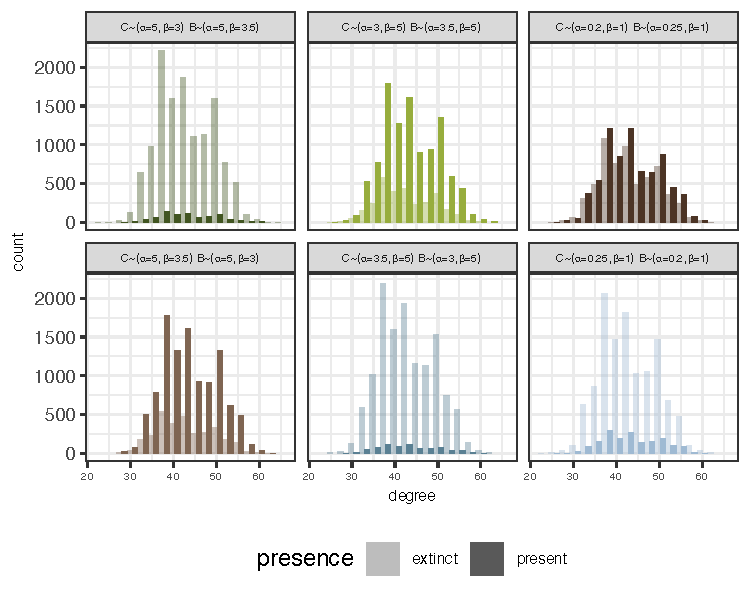
\includegraphics[width=0.65\textwidth]{../src/Code/R/Paulinha/figures/degree_distributions.pdf}
    \caption{Initial degree distribution at the beginning of the simulation, accounting for species that survived (darker colors) and species that went extinct (light colors). These sets of simulations considered random networks with 115 nodes (50 on one set and 65 on the other set and expected connectance of $p=0.65$) with 100 replicates for each parameter combination. Each panel presents a different combination of parameters for the distribution of costs (C) and benefits (B).}
    \label{fig:degree}
\end{figure}

\subsection{Effect of connectance}\label{effect-of-connectance}

Connectance (number of realized interactions given all possible
interactions) can influence dynamics, from the time it takes for
dynamics to stabilize to the final number of surviving species. The
number of time steps it takes for species' number to stabilize does not
depend on network connectance nor on specific parameterization of the
beta distribution describing costs and benefits. The mean time across
all simulations is \(3.75\) with a standard deviation ranging from
\(sd = 1.66-2.52\).

\begin{figure}[h]
    \centering
    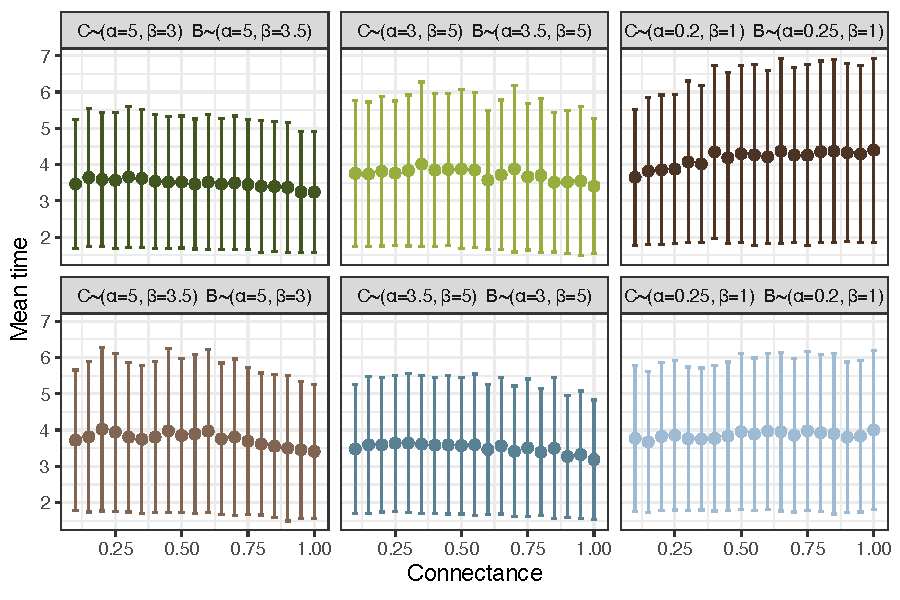
\includegraphics[width=0.65\textwidth]{../src/Code/R/Paulinha/figures/mean_time.pdf}
    \caption{Mean (and standard deviation) of the number of time steps until dynamics stabilize, i.e. no changes in the number of species in the community, as a function of network connectance.}
    \label{fig:meantime}
\end{figure}

The final proportion of surviving species, however, is sensitive to both
parameter combination underlying interactions and the connectance of the
network. When costs are greater than benefits (panels, 1, 5 and 6 in
Figure \ref{fig:sp_connectance}) increasing connectance decreases the
final number (proportion) of surviving species. When benefits are
slightly higher than costs (panels 2,3, and 4 in Figure
\ref{fig:sp_connectance}) increasing connectance in the system favors a
greater proportion of surviving species.

\begin{figure}[h!]
    \centering
    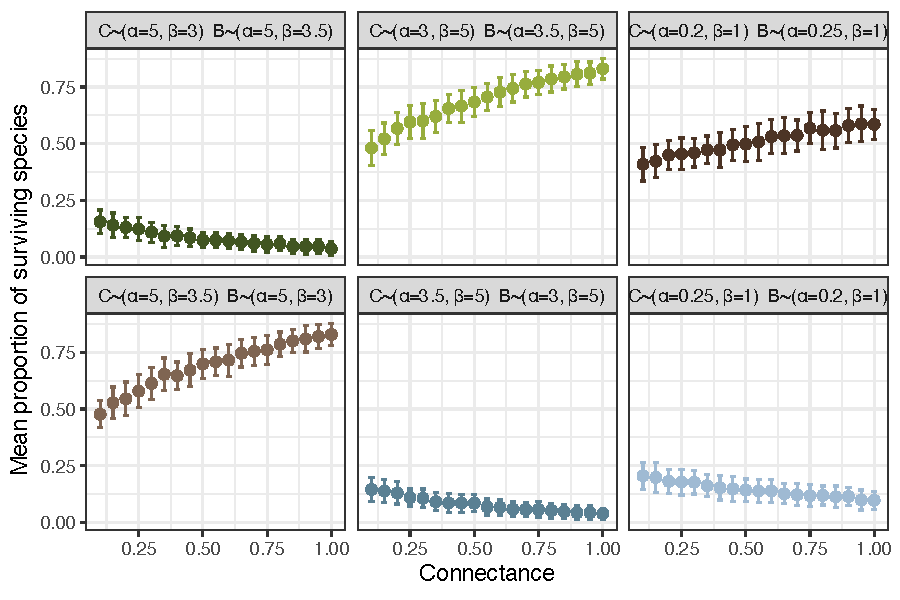
\includegraphics[width=0.65\textwidth]{../src/Code/R/Paulinha/figures/mean_prop_spp.pdf}
    \caption{Proportion of surviving species as a function of network connectance.}
    \label{fig:sp_connectance}
\end{figure}

\newpage

\subsubsection{Notes on references}\label{notes-on-references}

(Keyes et al. 2021) Comparison of food web robustness and the services
they provide, investigating factors that determine service response to
secondary extinctions. They have seven different services (wave
attenuattion, soreline stabilization, carbon sequestration, water
filtration, fishery, birdwatching, and waterfowl hunting). Species in
the food web are divided into ecosystem service providers and supporting
species. They explore 12 extinctions scenarios. Their key findings: (i)
food web and service robustness are highly correlated; (ii) service
robustness varies with trophic level and redundancy; (iii) species
providing services \textbf{do not} play a critical role in stabilizing
food webs; (iv) important supporting species are critical for both food
and service robustness.

(Ross et al. 2021) robustness of ecosystem services to species loss
using a ``qualitative Boolean framework''. The drivers of robustness are
features of the network that link species to the functions though
functional traits. Species are ``aggregated'' into functional traits
that in turn contribute to ecosystem service. Service is binary and
present as long as there's one species with a given functional trait the
service is present. They explore bipartite networks with a random
structure as well as pollination and seed dispersal networks.

\subsubsection{Follow-up questions}\label{follow-up-questions}

How is the robustness of food webs related to the ecosystem services
they provide? (Keyes et al. 2021) explored the consequences of secondary
extinctions to the maintenance of services in a food web system. They
found that food web and service robustness are highly correlated but
service robustness is dependent on trophic level. Additionally, they
also found that species providing services \textbf{do not} necessarily
play a critical role in stabilizing food webs and that species that play
supporting roles in service are the critical ones to robustness (of food
webs and services). How dependent are these results to the underlying
system providing the service? In their case, services are provided
through a food web, should we expect different results for pollination
or seed dispersal systems? In other words \emph{how does the nature of
the underlying ecological system influences the robustness of ecosystem
services they provide?}

\subsection{Supplementary Material}\label{supplementary-material}

\subsubsection{Boundary conditions for costs and benefits and the
persistence/extinction of
species}\label{boundary-conditions-for-costs-and-benefits-and-the-persistenceextinction-of-species}

What are the boundary conditions for the expectation of having all
species present (\(benefits > costs\)) and for having all species
extinct of the system (i.e., when \(benefits < costs\))? In other words,
we want to know what is the probability of having the benefits surpass
the costs, resulting in all species present in the network, and
alternatively, what is the probability of having all species removed
from the network if the costs of interaction surpass their benefits. The
solution to this problem, considering costs and benefits distributed
following independent beta distributions, relies on Appell F1
Hypergeometric function and was derived by Pham-Gia, Turkkan, and Eng
(1993). Since the Boolean function determining whether a species will be
present is given by a positive fitness, this can be achieved by a
species having greater benefits than costs for its interactions
(i.e.~\(\theta_b > \theta_c\)), with
\(\theta_b = X_1 \sim Beta(\alpha_1, \beta_1)\) and
\(\theta_c = X_2 \sim Beta(\alpha_2, \beta_2)\). We want to determine
the distribution of the difference \(\theta_d = \theta_b - \theta_c\).
This difference is piece wise and given by ((Pham-Gia, Turkkan, and Eng
1993)):

Considering \(A = Beta(\alpha1, \beta_1) \cdot Beta(\alpha_2, \beta_2)\)
and \(\cdot\) a product.

For \(-1 \leq \theta_d < 0\), meaning costs are greater than benefits,
we have: \[
p(\theta_d) = Beta(\alpha_2, \beta_1)\theta_d^{\beta1+\beta2-1}(1-\theta_d)^{\alpha_2+\beta_1-1} \cdot \\
                F_1(\beta_1, \alpha_1+\beta_1+\alpha_2+\beta_2-2, 1-\alpha_1; \beta_1+\alpha_2; 1-\theta_d, 1-\theta_d^2)/A
\] For \(0 < \theta_d \leq 1\), with benefits greater than costs, we
have: \[
p(\theta_d) = Beta(\alpha_1, \beta_2)\theta_d^{\beta_1+\beta_2-1}(1-\theta_d)^{\alpha_1\beta_2-1} \cdot \\
                F_1(\beta_2, 1-\alpha_2, \alpha_1+\beta_1+\alpha_2+\beta+2-2; \alpha_1+\beta_2; 1-\theta_d^2, 1+\theta_d)/A
\]

And finally, when the difference between the distribution of benefits
and costs is zero \(\theta_d = 0\) with \(\alpha_1 + \alpha_2 >1\) and
\(\beta_1 + \beta_2 >1\) we have:

\[
  p(\theta_d) = \frac{Beta(\alpha_1 + \alpha+2 -1, \beta_1+\beta_2-1)}{A}
\] \(F_1\) is the \textit{Appell $F_1$ Hypergeometric Function} with the
following form:

\[
F_1(a, b_1, b_2; c;x,y) = \sum_{m-n=0}^\infty \frac{(a)_{m+n}(b_1)_m(b_2)n}{(c)_{m+n} m!n!}x^my^n
\] with \((q)_m\) representing the Pochhammer symbol, indicating the
rising factor. Substituting the parameters, for the negative case
(\(-1 \leq \theta_d < 0\)) the parameters are \(a=\beta_1\),
\(b_1 = \alpha_1+\beta_1+\alpha2+\beta_2-2\), \(b_2 = 1-\alpha_1\);
\(c = \beta_1+\alpha_2\); \(x=1-\theta_2\), \(y= 1-\theta_d^2\). For the
negative case (\(0 < \theta_d \leq 1\)) the parameters are
\(a=\beta_2\), \(b_1 = 1-\alpha_2\),
\(b_2 = \alpha_1+\beta_1+\alpha2+\beta_2-2\), ;
\(c = \alpha_1+\beta_2\); \(x=1-\theta_2^2\), \(y= 1+\theta_d\).

\subsubsection{Other potential
distributions}\label{other-potential-distributions}

The choice of the beta distribution is supported by biological arguments
but it is still an arbitrary choice. Other possible distributions of
costs and benefits include:

\paragraph{Lognormal distribution}\label{lognormal-distribution}

As costs and benefits should, in principle, have the same sign, it is
more appropriate to use a distribution defined for positive values. The
derivation for the lognormal distribution is not as straight forward as
the one for the normal distribution, given we are interested in the
difference between two i.i.d. random variables drawn from a lognormal
distribution. One solution to find the probability that all species are
present is through numerical integration assuming both values are drawn
from \(lnN(0,1)\).

Alternatively, (Parham 2023) proposes a solution describing the
Difference-of-Log-Normals (DLN), characterizing its PDF, CDF, moments
and parameter estimators.

\begin{figure}[H]

{\centering 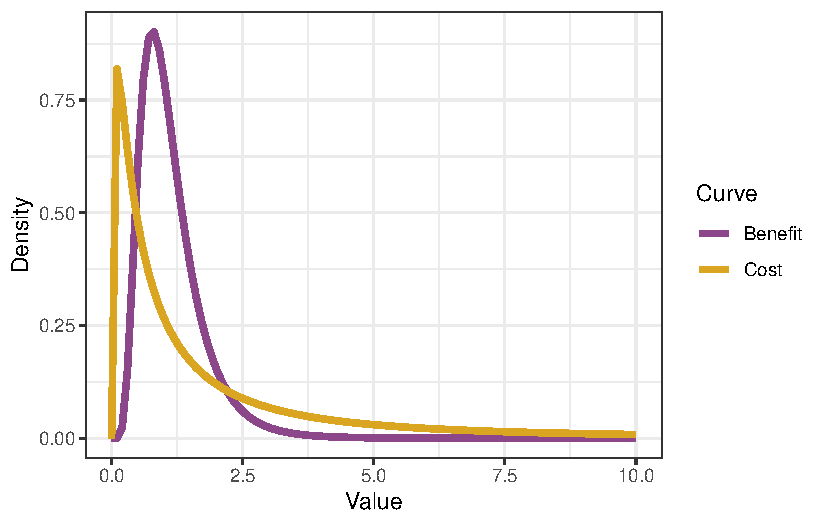
\includegraphics[width=0.5\linewidth,height=\textheight,keepaspectratio]{Notes_Paulinha_files/figure-pdf/lognormal-1.pdf}

}

\caption{Costs and benefits drawn from a lognormal distribution}

\end{figure}%

\paragraph{Normal distribution}\label{normal-distribution}

Assuming normally and independently distributed costs
\(C \sim N(\mu_c, \sigma^2_c)\) and benefits
\(B \sim  N(\mu_{b}, \sigma^2_b)\), we want first to know \(P(B>C)\).

\[
\begin{aligned}
P(B>C) = P(B-C > 0) \\
       = 1 - P(B-C \le 0) \\
\end{aligned}
\] If \(B\) and \(C\) are independent and normally distributed so is
their difference, with the expectation of their mean as
\(\mathbb{E}(B -C) = \mathbb{E} (B) - \mathbb{E}(C) = \mu_b - \mu_c = \mu\)
and of their variance as
\(Var(B-C) = \sigma^2_b + \sigma^2_c = \sigma\). Now we subtract the
mean and divide by the variance so that our difference is normally
distributed with \(\mu = 0\) and \(\sigma^2 = 1)\) such that
\(\frac{B-C-\mu}{\sigma} \sim N(0,1)\). And so:

\begin{equation} \label{eq:probs}
 P(B>C) = 1- \Phi \left(\frac{-\mu}{\sigma} \right)
\end{equation}

where \(\Phi\) is the cumulative distribution function of \(N(0,1)\).

Now let's consider an example: if species benefits have the distribution
\(B \sim N(1.2,2)\) and costs are distributed as \(C \sim N(2,1.5)\),
the distribution describing these values is:

\begin{figure}[H]

{\centering 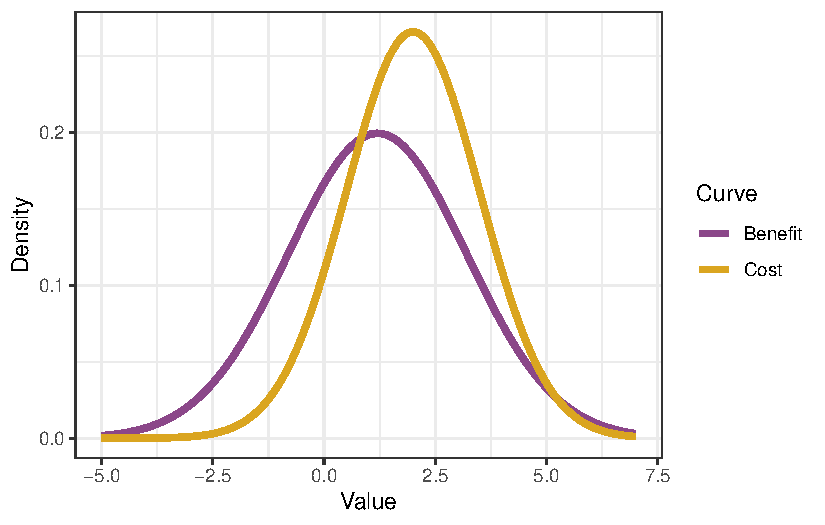
\includegraphics[width=0.5\linewidth,height=\textheight,keepaspectratio]{Notes_Paulinha_files/figure-pdf/functions-1.pdf}

}

\caption{Example of cost-benefit functions following a normal
distribution}

\end{figure}%

Using the derived expression, the resulting probability of having all
species present in this system, i.e., the \(P(B>C)\), meaning benefits
are greater than costs is: 0.3344646. Alternatively, the probability
that all species goes extinct in this example is: 0.6655354.

In more general terms, we can explore how the difference between
benefits and costs influences the probability of all species coexisting.
Assuming a standard deviation of \(\sigma^2 = 1\) we explore the effect
of the mean difference between costs and benefits in species'
probability of persistence, deriving the probability according to
equation \ref{eq:probs}.

\begin{figure}[H]

{\centering 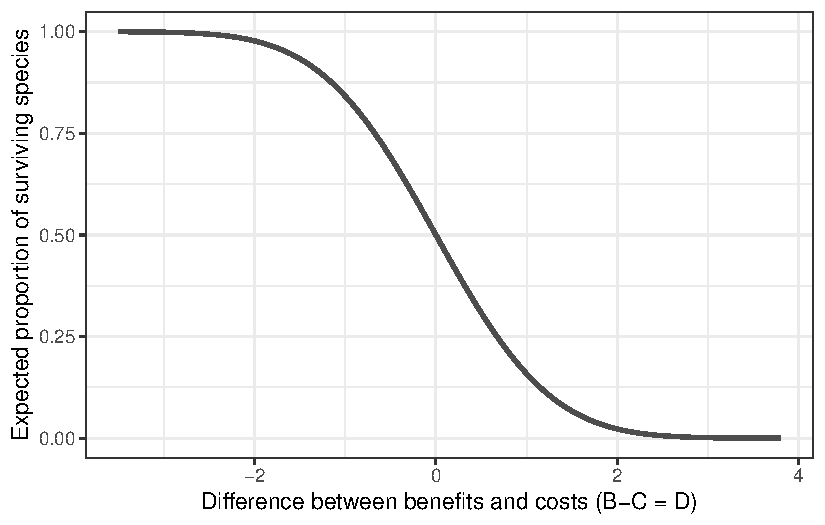
\includegraphics[width=0.5\linewidth,height=\textheight,keepaspectratio]{Notes_Paulinha_files/figure-pdf/coexistence-1.pdf}

}

\caption{Expected proportion of species' persistence given the
difference in benefits and costs}

\end{figure}%

\newpage

\subsection*{References}\label{references}
\addcontentsline{toc}{subsection}{References}

\phantomsection\label{refs}
\begin{CSLReferences}{1}{0}
\bibitem[\citeproctext]{ref-cattin2004phylogenetic}
Cattin, Marie-France, Louis-Félix Bersier, Carolin Banašek-Richter,
Richard Baltensperger, and Jean-Pierre Gabriel. 2004. {``Phylogenetic
Constraints and Adaptation Explain Food-Web Structure.''} \emph{Nature}
427 (6977): 835--39.

\bibitem[\citeproctext]{ref-dunne2008compilation}
Dunne, Jennifer A, Richard J Williams, Neo D Martinez, Rachel A Wood,
and Douglas H Erwin. 2008. {``Compilation and Network Analyses of
Cambrian Food Webs.''} \emph{PLoS Biology} 6 (4): e102.

\bibitem[\citeproctext]{ref-fowler2010extinction}
Fowler, Mike S. 2010. {``Extinction Cascades and the Distribution of
Species Interactions.''} \emph{Oikos} 119 (5): 864--73.

\bibitem[\citeproctext]{ref-keyes2021ecological}
Keyes, Aislyn A, John P McLaughlin, Allison K Barner, and Laura E Dee.
2021. {``An Ecological Network Approach to Predict Ecosystem Service
Vulnerability to Species Losses.''} \emph{Nature Communications} 12 (1):
1586.

\bibitem[\citeproctext]{ref-parham2023difference}
Parham, Robert. 2023. {``The Difference-of-Log-Normals Distribution:
Properties, Estimation, and Growth.''} \emph{arXiv Preprint
arXiv:2302.02486}.

\bibitem[\citeproctext]{ref-pham1993bayesian}
Pham-Gia, Thu, Noyan Turkkan, and P Eng. 1993. {``Bayesian Analysis of
the Difference of Two Proportions.''} \emph{Communications in
Statistics-Theory and Methods} 22 (6): 1755--71.

\bibitem[\citeproctext]{ref-ross2021universal}
Ross, Samuel RP-J, Jean-François Arnoldi, Michel Loreau, Cian D White,
Jane C Stout, Andrew L Jackson, and Ian Donohue. 2021. {``Universal
Scaling of Robustness of Ecosystem Services to Species Loss.''}
\emph{Nature Communications} 12 (1): 5167.

\bibitem[\citeproctext]{ref-stouffer2005quantitative}
Stouffer, Daniel B, José Camacho, Roger Guimera, CA Ng, and LA Nunes
Amaral. 2005. {``Quantitative Patterns in the Structure of Model and
Empirical Food Webs.''} \emph{Ecology} 86 (5): 1301--11.

\end{CSLReferences}




\end{document}
